\documentclass[12pt,border=1mm]{standalone}
\usepackage[utf8]{inputenc}
\usepackage[usenames,x11names]{xcolor}
\usepackage[x11names]{xcolor}
\colorlet{ctrlcol}{DeepSkyBlue1}

\usepackage{tikz}
\usetikzlibrary{circuits.logic.IEC}
\usetikzlibrary{arrows,arrows.meta}

\begin{document}
	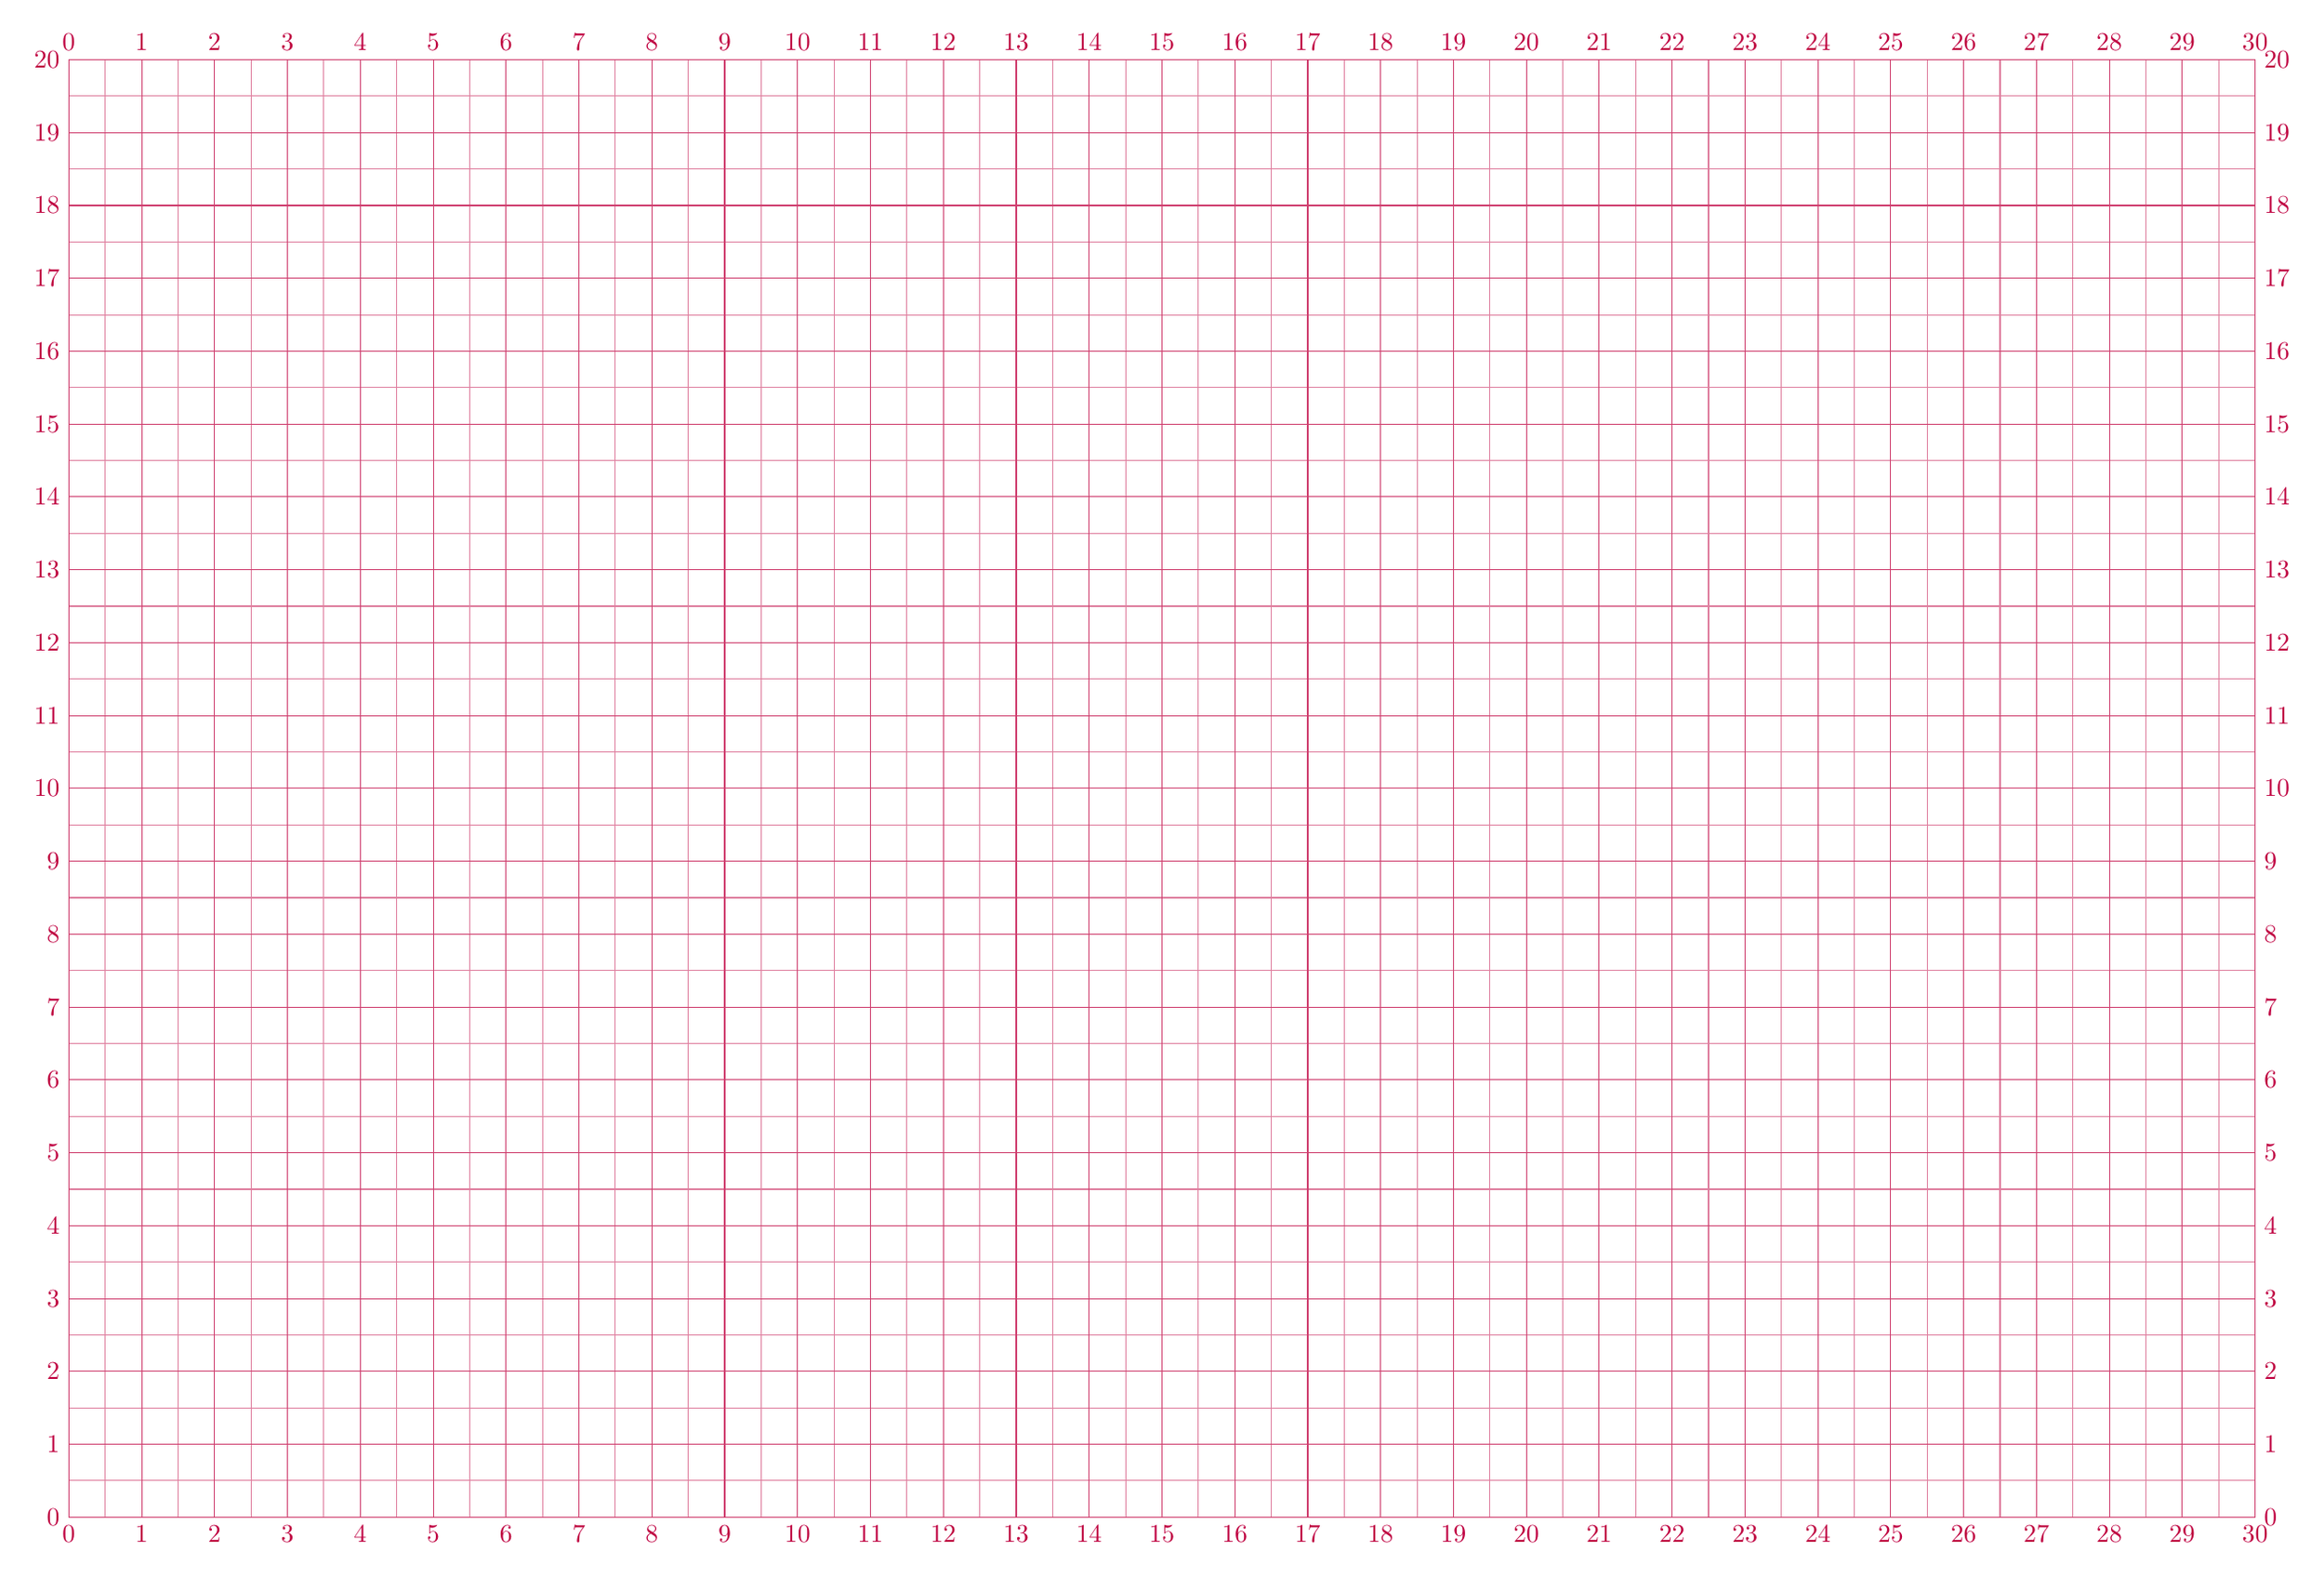
\begin{tikzpicture}[%
		large circuit symbols,
		circuit logic IEC,
		circuit symbol lines/.style={draw, very thick},
		font=\sffamily,
		>=Latex
		]

		%% Hilfslinien. Zeilen auskommentieren, um Hilfslinien zu entfernen!
		
		\draw [thin,purple,opacity=0.5,step=0.5cm] (0,0) grid (30,20);
		\draw [purple,opacity=0.5] (0,0) grid (30,20);
		\foreach \x in {0,...,20} {
			\draw [purple] (-0,\x) node[left]{$\x$};
			\draw [purple] (30,\x) node[right]{$\x$};
		}
		\foreach \x in {0,...,30} {
			\draw [purple] (\x,20) node[above]{$\x$};
			\draw [purple] (\x,0) node[below]{$\x$};
		}
		
		

	\end{tikzpicture}
\end{document}
